\documentclass{beamer}
\usecolortheme{wolverine}

% math stuff
\usepackage{amsmath}
\usepackage{amsthm}
\usepackage{amssymb}
\usepackage{xcolor}

\usepackage{float}
\usepackage{subcaption}

% to insert images
\usepackage{graphicx}

% to correctly insert stressed characters
\usepackage[T1]{fontenc}
\usepackage[utf8]{inputenc}

\usepackage{multirow}

% Bibliography
% \usepackage[style=alphabetic]{biblatex}
% \usepackage[nottoc]{tocbibind}
% \usepackage{bibentry}
% \setcounter{biburllcpenalty}{9000}
% \usepackage{nameref}
% \addbibresource{slides.bib}

% to put links in table of contents
\usepackage{hyperref}
\hypersetup{colorlinks=false, %set true if you want colored links
	linktoc=all,     %set to all if you
}

\usepackage{mathtools}

% Add symbols
% \usepackage{textcomp}

% Add command for Real and Z sets
% \usepackage{dsfont}
% \newcommand{\Rset}{$\mathds{R}$}
% \newcommand{\Zset}{$\mathds{Z}$}

% Code highlighting
% \usepackage{minted}
% \usemintedstyle{perldoc}
% \setminted{
%     frame=single,
%     breaklines,
% }

% tikz figures
% \usepackage{tikzit}
% \input{style.tikzstyles}

% number rounding
\usepackage{siunitx}
\sisetup{round-mode=places,round-precision=5}

\definecolor{myyellow}{RGB}{225, 225, 0}

\title{Thesis notes}
\date{11th May}

% any code between @(...)@ is escaped back to LaTeX
% \lstset{escapeinside={@(}{)@}}

% algorithms
\usepackage[ruled,vlined]{algorithm2e}
% \newtheorem{theorem}{Theorem}

\begin{document}

\frame{\titlepage}

\begin{frame}[c]
	\frametitle{The Echo Chamber Problem - notation}

	\begin{itemize}
		\item $G = (V, E ^{+}, E ^{-}) $ interaction graph
		\item $ \mathcal{C} $ set of contents
		\item $C \in \mathcal{C} $ content, $\mathcal{T} _{C} $ set of threads
		      associated with $C$. A thread $T \in \mathcal{T} _{C} $ is a
		      subgraph of $G$
		      % So $G = \bigcup _{C
		      % \in \mathcal{C} } \bigcup _{T \in \mathcal{T} _C} T $ union of all
		      % threads of all contents
		\item $U \subseteq V$ subset of users, $T[U]$ subgraph of $T$ induced
		      by $U$. $|T(U)|$ is the number of edges of this subgraph
	\end{itemize}
\end{frame}

\begin{frame}[c]
	\frametitle{The Echo Chamber Problem - notation}
	\begin{itemize}
		\item $\eta(C)$ fraction of negative edges associated with $C$
		      (analogous definition for a thread $T$). Content (or thread)
		      controversial if $\eta \in [\alpha, 1]$
		\item $\hat{\mathcal{C} } \subseteq \mathcal{C} $ set of \textit{controversial}
		      contents

		\item $\mathcal{S} _C (U)$ set of \textit{non controversial} threads
		      induced by $U$, for \textit{controversial} contents, i.e.

			      {\small
				      \begin{equation}
					      \mathcal{S} _{C} (U) = \{ T[U] \; s.t. \; T[U] \; non \;
					      controversial, T \in \mathcal{T} _{C}, C
					      \in \hat{\mathcal{C}}, U \subseteq V\}
				      \end{equation}
			      }
	\end{itemize}

\end{frame}

\begin{frame}[c]
	\frametitle{The Echo Chamber Problem}
	\textbf{Goal}: given an interaction graph $G$, find $U \subseteq V$ maximing

	\begin{equation}
		\xi (U) = \sum^{}_{C \in \hat{\mathcal{C}} } \sum^{}_{T[U] \in S_C (U)}
		| T[U] |
	\end{equation}

	The set of users maximing the expression is denoted as $\hat{U}$ and the
	corresponding score is $\xi(G)$
\end{frame}

\begin{frame}[c]
	\frametitle{The Densest Echo Chamber Problem}
	\textbf{Goal}: given an interaction graph $G$, find $U \subseteq V$ maximing

	\begin{equation}
		\psi (U) = \sum^{}_{C \in \hat{\mathcal{C}} } \sum^{}_{T[U] \in S_C (U)}
		\frac{| T[U] |}{|U|}
	\end{equation}

	The set of users maximing the expression is denoted as $\hat{U}$ and the
	corresponding score is $\psi(G)$
\end{frame}

\begin{frame}[c]
	\frametitle{Baseline datasets}
	Reddit datasets:

	\begin{itemize}
		\item r/asktrumpsupporters, where $> 40 \% $ of the nodes are labeled.
		      Labels: Supporter, NonSupporter, Undecided. Missing labels are
		      due to removed accounts and comments.
		\item r/debatereligion, where $\approx 1 \%$ of the nodes are labeled.
		      Labels: Christian, Muslim, ...

		      Missing labels are mostly due to custom labels chosen by the user.
	\end{itemize}

	In both cases users declare their "position" through flairs.
\end{frame}

\begin{frame}[c]
	\frametitle{Baseline datasets}
	\begin{itemize}
		\item Look at the accounts a user is following
		      \begin{figure}[htpb]
			      \centering
			      
\includegraphics[width=0.6\linewidth]{img/following_cortez.png}
		      \end{figure}
		\item Use the account name to look at the political party on
		      wikipedia

		      \begin{figure}[htpb]
			      \centering
			      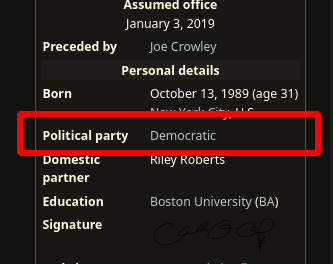
\includegraphics[width=0.4\linewidth]{img/cortez_wikipedia.png}
		      \end{figure}

	\end{itemize}
\end{frame}

\begin{frame}[c]
	\frametitle{Baseline datasets}
	Use the party of the majority of the people a user is following for
	labeling him.

	\begin{enumerate}
		\item Construct the \emph{Interaction graph} from @nytimes (or any other
		      profile)
		\item select k-core for reducing the number of users
		\item label the nodes in the k-core
	\end{enumerate}

	\begin{itemize}
		\item For 200 contents from @nytimes the 4-core contains $\approx 1000$
		      nodes, and around $50 \%$ of them is labeled
		\item of these labeled nodes, $80 \%$ is labeled as democrat and
		      the remaining $20 \%$ as republican
	\end{itemize}

\end{frame}

\begin{frame}[c]
	\frametitle{Baseline results}

	\begin{figure}
		\begin{center}
			\begin{subfigure}[b]{0.4\textwidth}
				\centering
				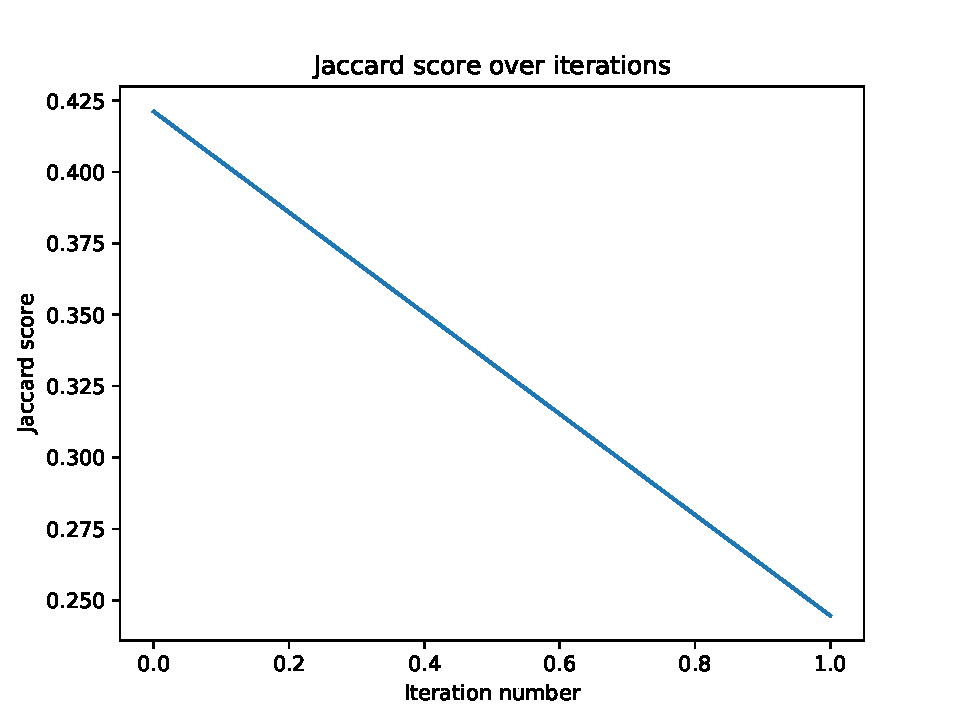
\includegraphics[width=\textwidth]{out/nytimes_baseline200/jaccard_iterations.pdf}
			\end{subfigure}
			\begin{subfigure}[b]{0.4\textwidth}
				\centering
				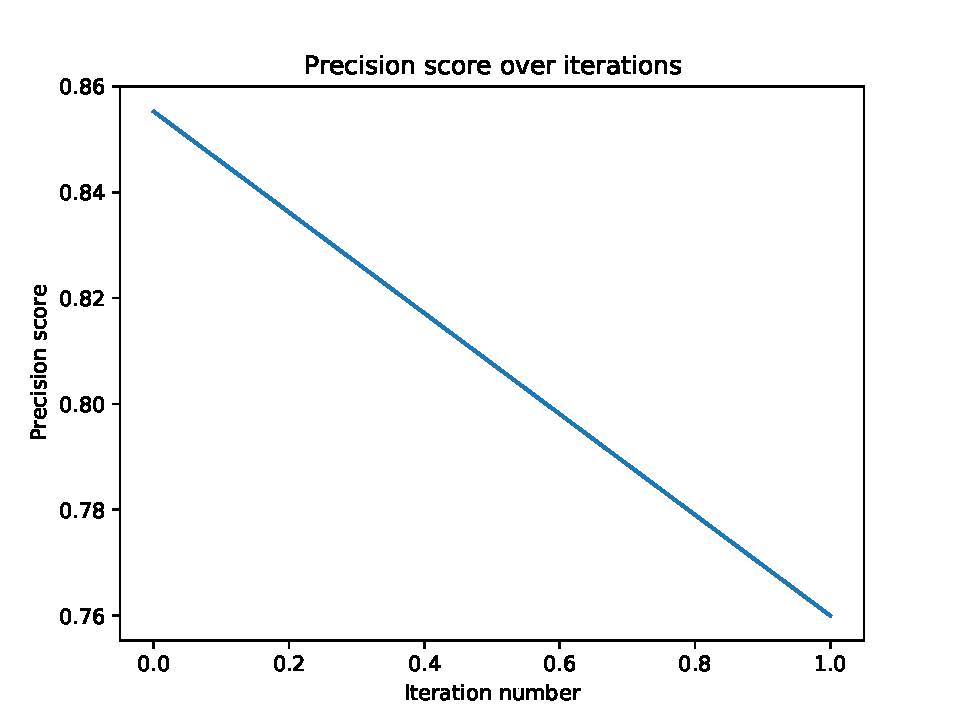
\includegraphics[width=\textwidth]{out/nytimes_baseline200/precision_iterations.pdf}
			\end{subfigure}
		\end{center}
	\end{figure}

	\begin{itemize}
		\item Adjusted RAND score: 0.004424665696313976
		\item RAND score: 0.44517376780167617
		\item Jaccard score: 0.17509727626459143
	\end{itemize}

	Dataset is skewed. Both in the first and second iteration the solution
	contains nodes whose majority is democrat

\end{frame}

% \begin{frame}[c]
%     \frametitle{Results}
%
%     The algorithm (even if it is just an approximation) requires a lot of times
%     even on smaller graphs.
%
%     \bigskip
%
%     For a graph with $100$ snapshots and $k = 10$, $|V| \approx 2000$ and $|E|
%         \approx 2000$ it needs $> 6 $ hours.
%
% \end{frame}

% \begin{frame}[c]
%     \frametitle{Results}
%
%     \tiny{
%         \begin{table}[htpb]
%             \centering
%             \caption{Echo chamber scores. For the $\xi_{round}(G) $ the results tuple
%                 corresponds to (score, $|U|$, number of contributing threads, time in
%                 seconds). In the other scores the number of contributing thread
%                 is omitted. $\alpha = 0.4$}
%             \begin{tabular}{c|c|c|c}
%                 \textbf{Source, $|V|$, $|E|$, $|\hat{\mathcal{C}}  |$} & $\xi_{round}(G) $ & $\psi_{Dens}(G)$ & $\psi_{T-Dest} (G)$ \\
%                 \hline
%                 nytimes, 20051, 24468, 44                              &
%                 (5961, 4814, 243, 400)                                 & (1.2, 16, 1000)   &
%                 (1.2, 16, 1000)                                                                                                     \\
%                 foxnews, 45509, 82494, 232                             &
%                 (50240, 26352, 1090, 24000)                            & (1.96, 28, 5000)  & (1.97,
%                 35, 5000)                                                                                                           \\
%             \end{tabular}
%         \end{table}
%     }
%
%     \tiny{
%         \begin{table}[htpb]
%             \centering
%             \caption{Echo chamber scores for alpha chosen as the median of the
%                 $\eta$ of the contents. Tuple meaning is the same as above}
%             \begin{tabular}{c|c|c|c}
%                 \textbf{Source, $|V|$, $|E|$, $|\hat{\mathcal{C}}  |$} & $\xi_{round}(G) $ & $\psi_{Dens}(G)$ & $\psi_{T-Dest} (G)$ \\
%                 \hline
%                 nytimes, 20051, 24468, 62                              &
%                 (7337, 5775, 288, 243, 400)                            & (1.2, 16, 1000)
%                                                                        & (1.2, 16, 1000)                                            \\
%                 foxnews, 45509, 82494, 154                             &
%                 (53643, 30816, 810, 24000)                             & (1.96, 28, 5000)  & (1.97,
%                 35, 5000)                                                                                                           \\
%             \end{tabular}
%         \end{table}
%     }
%
%     \small{
%         Median alpha for @nytimes: 0.358
%
%         Median alpha for @foxnews: 0.553
%     }
% \end{frame}

% \begin{frame}[c]
%     \frametitle{Choosing alpha}
%     It could be interesting to indagate the relationship between the Echo
%     Chamber Score and alpha for different datasets, also relating it to the
%     distribution of $\eta$ for the contents and threads.
%
%     \begin{figure}[htpb]
%         \centering
%         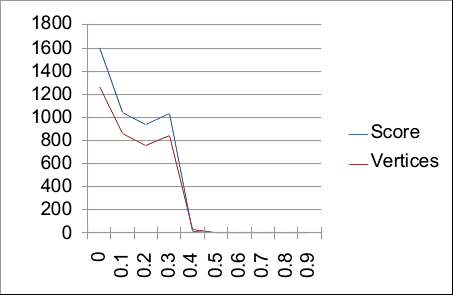
\includegraphics[width=0.6\linewidth]{img/cats_alpha_choice.png}
%         \label{fig:img/cats_alpha_choice}
%     \end{figure}
% \end{frame}

% \begin{frame}[c]
%     \frametitle{A model for the Echo Chamber Problem (1)}
%     Model parameters:
%     \begin{itemize}
%         \item $b_{i} $, the group of each user $i$
%         \item $\omega ^{+} _{rs} $ and $\omega ^{-} _{rs} $, the probabilities
%               of positive and negative edges, respectively, between users in
%               group $r$ and $s$ ($\omega ^{+} _{rs} + \omega ^{-} _{rs} \leq 1$).
%         \item $\theta$, controlling the reduction of probability of interacting
%               between \emph{inactive} communities
%     \end{itemize}
%
%     For each content:
%     \begin{enumerate}
%         \item Sample $n'$ among the $n$ communities. These are the
%               \emph{active} communities in the content discussion
%         \item For each node pairing $i, j$ consider their corresponding groups $r$ and
%               $s$.
%               \begin{itemize}
%                   \item If both communities are \emph{active} draw from the
%                         categorical distribution $(\omega _{rs} ^{+}, \omega
%                             _{rs} ^{-}, 1 - \omega _{rs} ^{+} - \omega _{rs} ^{-}) $ to add an edge (or
%                         not).
%                   \item Otherwise draw from the categorical $(\theta \omega _{rs} ^{+},
%                             \theta \omega
%                             _{rs} ^{-}, 1 - \theta (\omega _{rs} ^{+} + \omega _{rs}
%                             ^{-}))$, $\theta \leq 1$.
%               \end{itemize}
%
%     \end{enumerate}
%
% \end{frame}

% \begin{frame}[c]
%     \frametitle{A model for the Echo Chamber Problem}
%     Again each node has a group assignment and there are probabilities of
%     positive and negative edges $\omega _{rs}^{+}  $ and $\omega _{rs}^{+}  $,
%     respectively.
%
%     \begin{enumerate}
%         \item Generate the \emph{follow} graph $G$ by using a SBM with parameters
%               $\{ \phi _{rs}  \}$.
%         \item Each node can be active with probability $\beta_{a}  $
%         \item Any active node activates his inactive neighbours in $G$ with
%               probability $\beta_n$
%               % \item Let $a_{i} $ be the number of \emph{active} neighbours of node
%               %     $i$ in $G$ and $m_{i} $ the number of neighbours of node $i$ in
%               %     $G$. Any node inactive from the previous step is activated with
%               %     probability $ \frac{a_i}{m_i} \beta _{n} $
%         \item active nodes interact according to the categorical $(\omega _{rs}
%                   ^{+}, \omega _{rs} ^{-}, 1 - \omega _{rs} ^{+} - \omega _{rs} ^{-})
%               $ otherwise (at least one of the 2 nodes is inactive) with
%               categorical $(\theta \omega _{rs} ^{+}, \theta \omega _{rs} ^{-}, 1
%                   - \theta (\omega _{rs} ^{+} + \omega _{rs} ^{-}))$, $\theta \leq 1$
%     \end{enumerate}
%
% \end{frame}

% \begin{frame}[c]
%     \frametitle{Computing the score on the synthetic data (5)}
%     Third graph: much smaller distinction in the interaction between
%     communities.
%
%     \begin{figure}
%         \begin{center}
%             \begin{subfigure}[b]{0.3\textwidth}
%                 \centering
%                 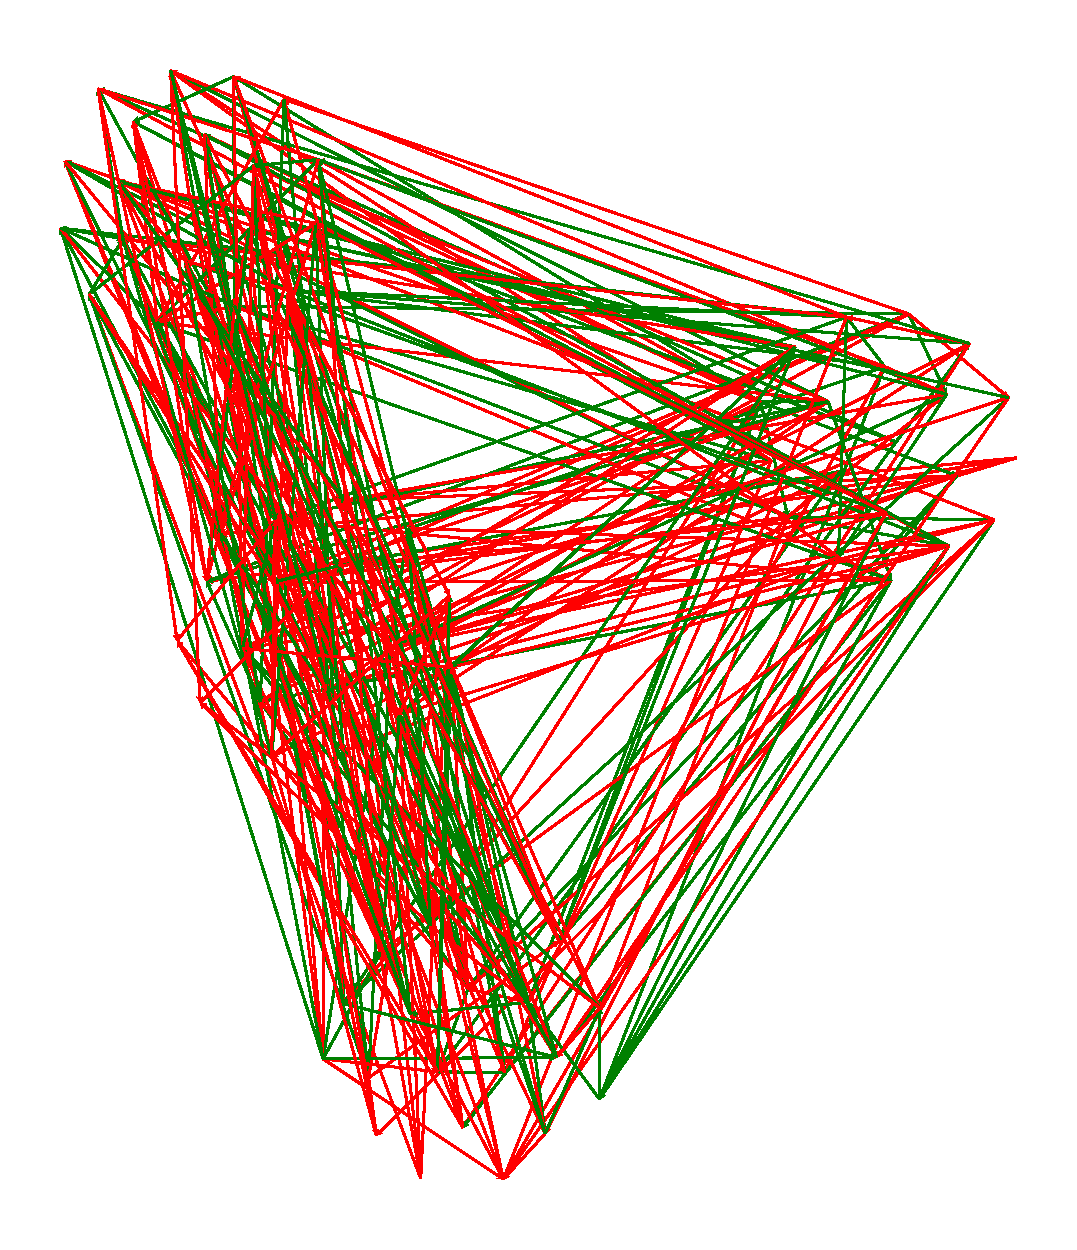
\includegraphics[width=\textwidth]{out/synthetic/model2_graph2.pdf}
%                 \caption{Graph}
%                 \label{fig:}
%             \end{subfigure}
%             \begin{subfigure}[b]{0.3\textwidth}
%                 \centering
%                 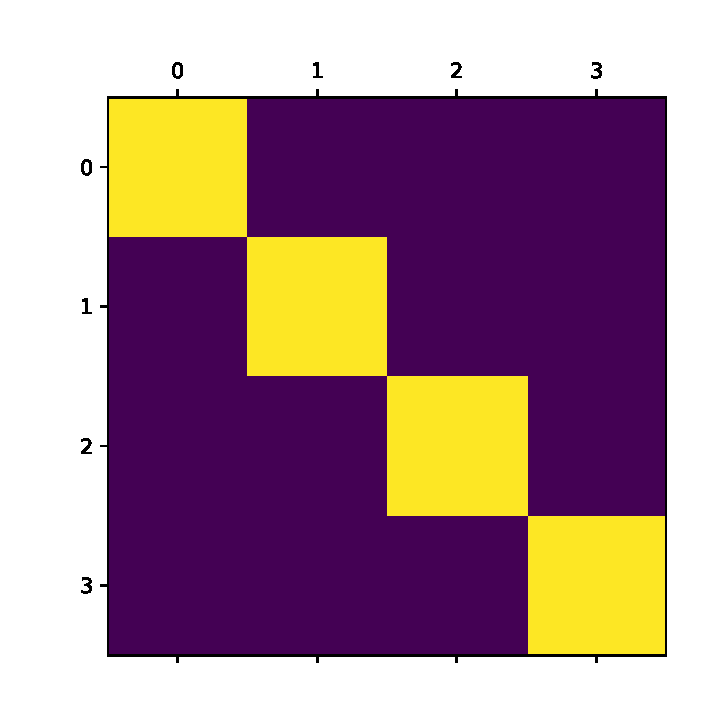
\includegraphics[width=\textwidth]{out/synthetic/model2_omega_positive3.pdf}
%                 \caption{$\omega ^{+} _{rs} $}
%                 \label{fig:out/synthetic/omega_positive1.pdf}
%             \end{subfigure}
%             \begin{subfigure}[b]{0.3\textwidth}
%                 \centering
%                 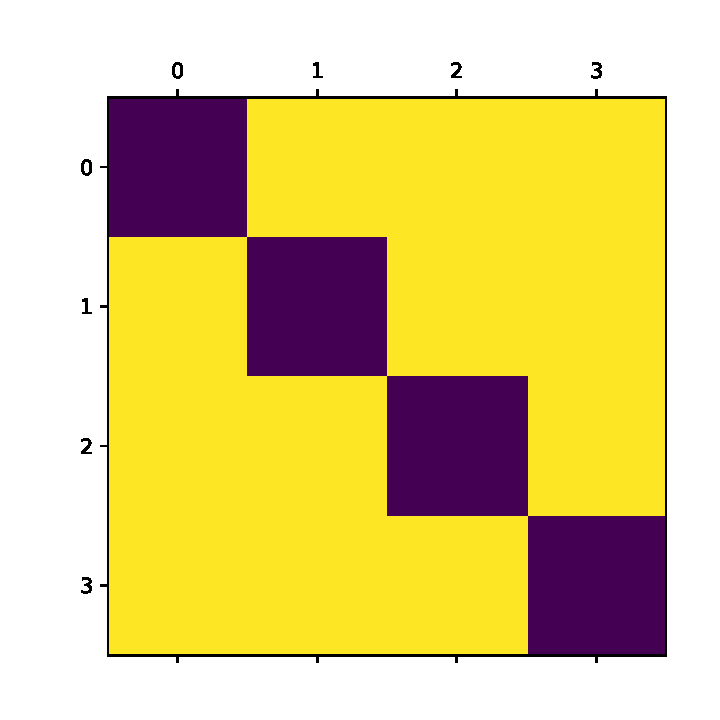
\includegraphics[width=\textwidth]{out/synthetic/model2_omega_negative3.pdf}
%                 \caption{$\omega ^{-} _{rs} $}
%                 \label{fig:}
%             \end{subfigure}
%         \end{center}
%     \end{figure}
%
%     $|V| = 80, \; |E| \approx 400, \; \eta(G) \approx 0.58, \; \bar{\xi}(G)
%         \approx 25$.
%
%     Rand $= 0.6$, adjusted Rand $= 0.007$
% \end{frame}

\begin{frame}[c]
	\frametitle{Relationship between alpha and Echo Chamber Score}
	\begin{figure}
		\begin{center}
			\begin{subfigure}[b]{0.3\textwidth}
				\centering
				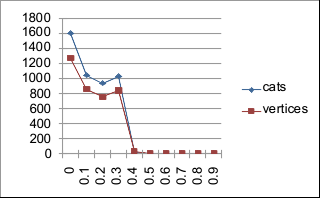
\includegraphics[width=\textwidth]{out/alpha/cats_alpha.png}
				\caption{r/cats}
				\label{fig:out/alpha/cats_alpha.png}
			\end{subfigure}
			\begin{subfigure}[b]{0.3\textwidth}
				\centering
				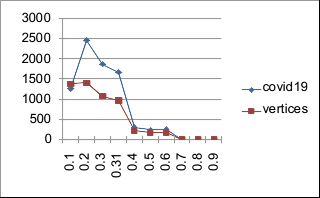
\includegraphics[width=\textwidth]{out/alpha/covid19_alpha.png}
				\caption{r/covid19}
				\label{fig:out/alpha/covid19_alpha.png}
			\end{subfigure}
			\begin{subfigure}[b]{0.3\textwidth}
				\centering
				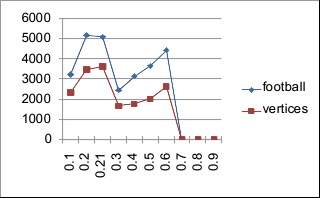
\includegraphics[width=\textwidth]{out/alpha/football_alpha.png}
				\caption{r/football}
				\label{fig:out/alpha/football_alpha.png}
			\end{subfigure}
		\end{center}
	\end{figure}

	\begin{figure}
		\begin{center}
			\begin{subfigure}[b]{0.3\textwidth}
				\centering
				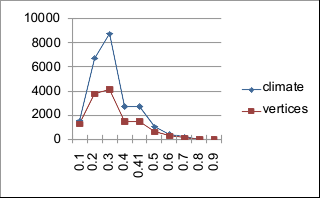
\includegraphics[width=\textwidth]{out/alpha/climate_alpha.png}
				\caption{r/climate}
				\label{fig:out/alpha/climate_alpha.png}
			\end{subfigure}
			\begin{subfigure}[b]{0.3\textwidth}
				\centering
				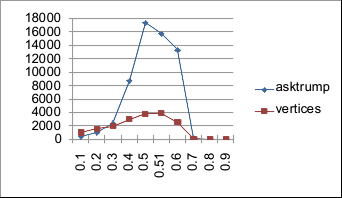
\includegraphics[width=\textwidth]{out/alpha/asktrump_alpha.png}
				\caption{r/asktrumpsupporters}
				\label{fig:out/alpha/asktrump_alpha.png}
			\end{subfigure}
			\begin{subfigure}[b]{0.3\textwidth}
				\centering
				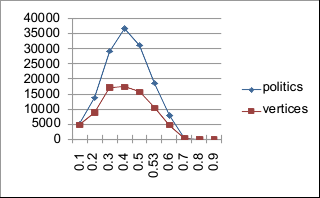
\includegraphics[width=\textwidth]{out/alpha/politics_alpha.png}
				\caption{r/politics}
				\label{fig:out/alpha/politics_alpha.png}
			\end{subfigure}
		\end{center}
	\end{figure}



\end{frame}

\begin{frame}[c]
	\frametitle{Analyzing @foxnews results}
	A graph from @foxnews, with 300 contents

	$\alpha $ chosen as the median of the $\eta$ of the contents, $\alpha =
		0.58$.

	The graph contains 21004 nodes and 44441 edges, $\xi(G) = 17473 $ on 10017
	vertices and define $598$ components. In the original graph they were part
	of the same component.

	\begin{itemize}
		\item Average shortest path length: 1.031
		\item Median shortest path length: 1.0
		\item Average degree: 1.7
		\item Contributing threads: 155
		\item Number of threads: 320
	\end{itemize}

\end{frame}

\begin{frame}[c]
	\frametitle{Analyzing @foxnews results}

	\begin{figure}
		\begin{center}
			\begin{subfigure}[b]{0.4\textwidth}
				\centering
				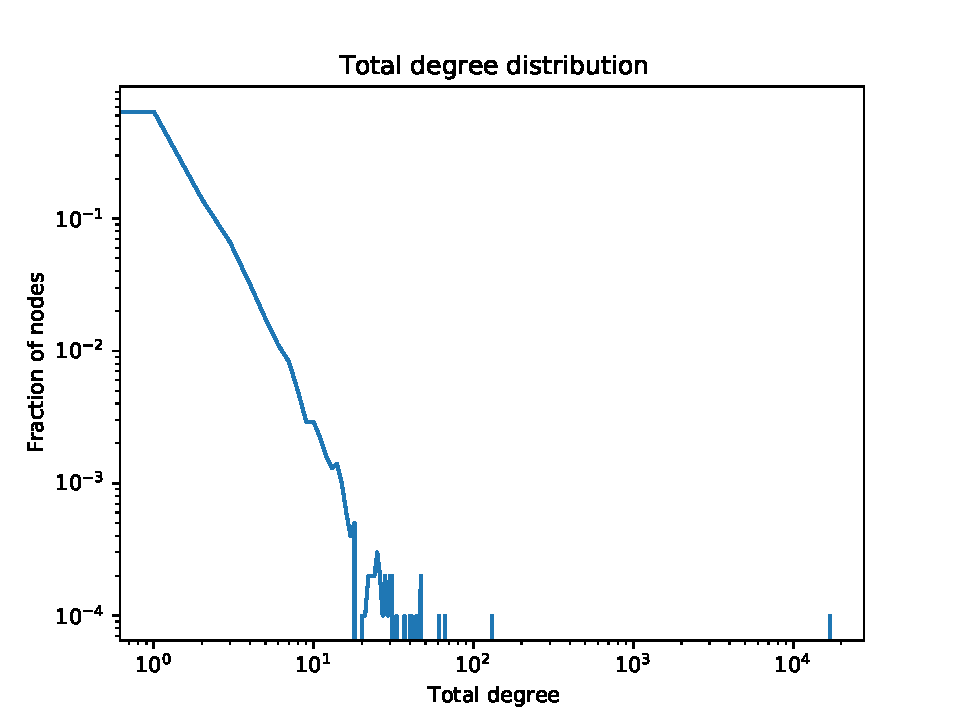
\includegraphics[width=\textwidth]{out/foxnews4000/results/degree-total-dist.pdf}
				\caption{total degree distribution}
				\label{fig:out/foxnews4000/results/degree-total-dist.pdf}
			\end{subfigure}
			\begin{subfigure}[b]{0.4\textwidth}
				\centering
				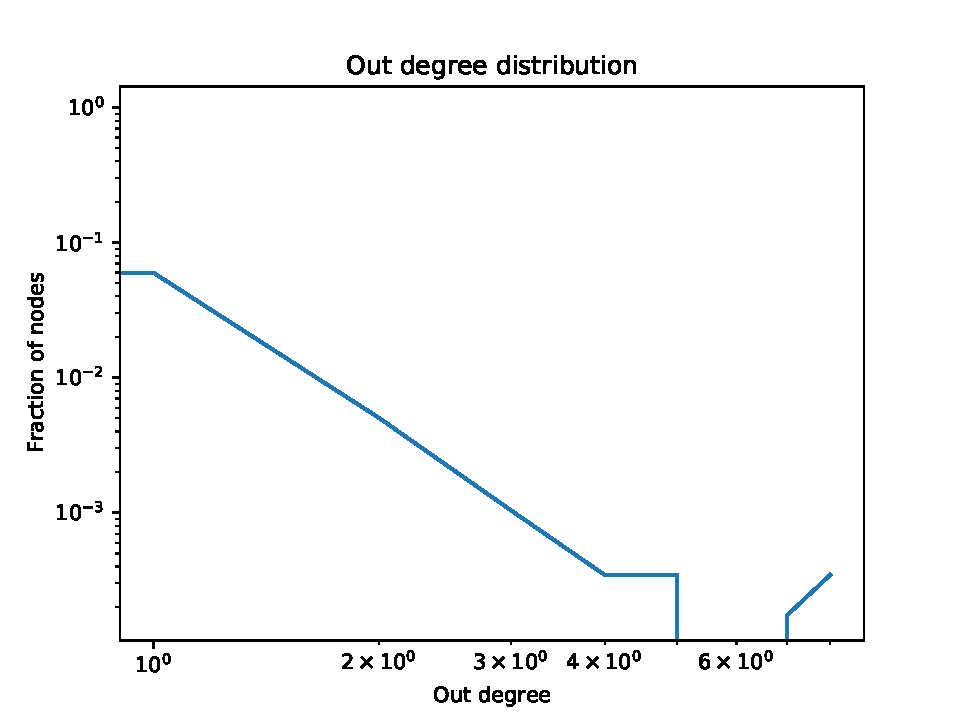
\includegraphics[width=\textwidth]{out/results/degree-out-dist.pdf}
				\caption{out degree distribution}
				\label{fig:}
			\end{subfigure}
		\end{center}
	\end{figure}


\end{frame}

\begin{frame}[c]
	\frametitle{Analyzing @foxnews results}
	Threads that contribute the most to the score:
	\begin{figure}[htpb]
		\centering
		
\includegraphics[width=0.5\textwidth]{out/foxnews4000/results/thread1.png}
		\caption{975}
		\label{fig:name}
	\end{figure}
	\begin{figure}[htpb]
		\centering
		
\includegraphics[width=0.5\textwidth]{out/foxnews4000/results/thread2.png}
		\caption{870}
		\label{fig:name}
	\end{figure}
	\begin{figure}[htpb]
		\centering
		
\includegraphics[width=0.5\textwidth]{out/foxnews4000/results/thread3.png}
		\caption{803}
		\label{fig:name}
	\end{figure}


\end{frame}

\end{document}
